\chapter{Background}

\section{Emotion Representation in LLMs}

\subsection{Discrete Emotion Labels and Their Limitations}

Early work treated emotion as a small set of discrete categories. The most influential taxonomy is Ekman's seven basic emotions: anger, contempt, disgust, enjoyment, fear, sadness, and surprise~\cite{ekman1999basic}. 

\begin{figure}[H]
    \centering
    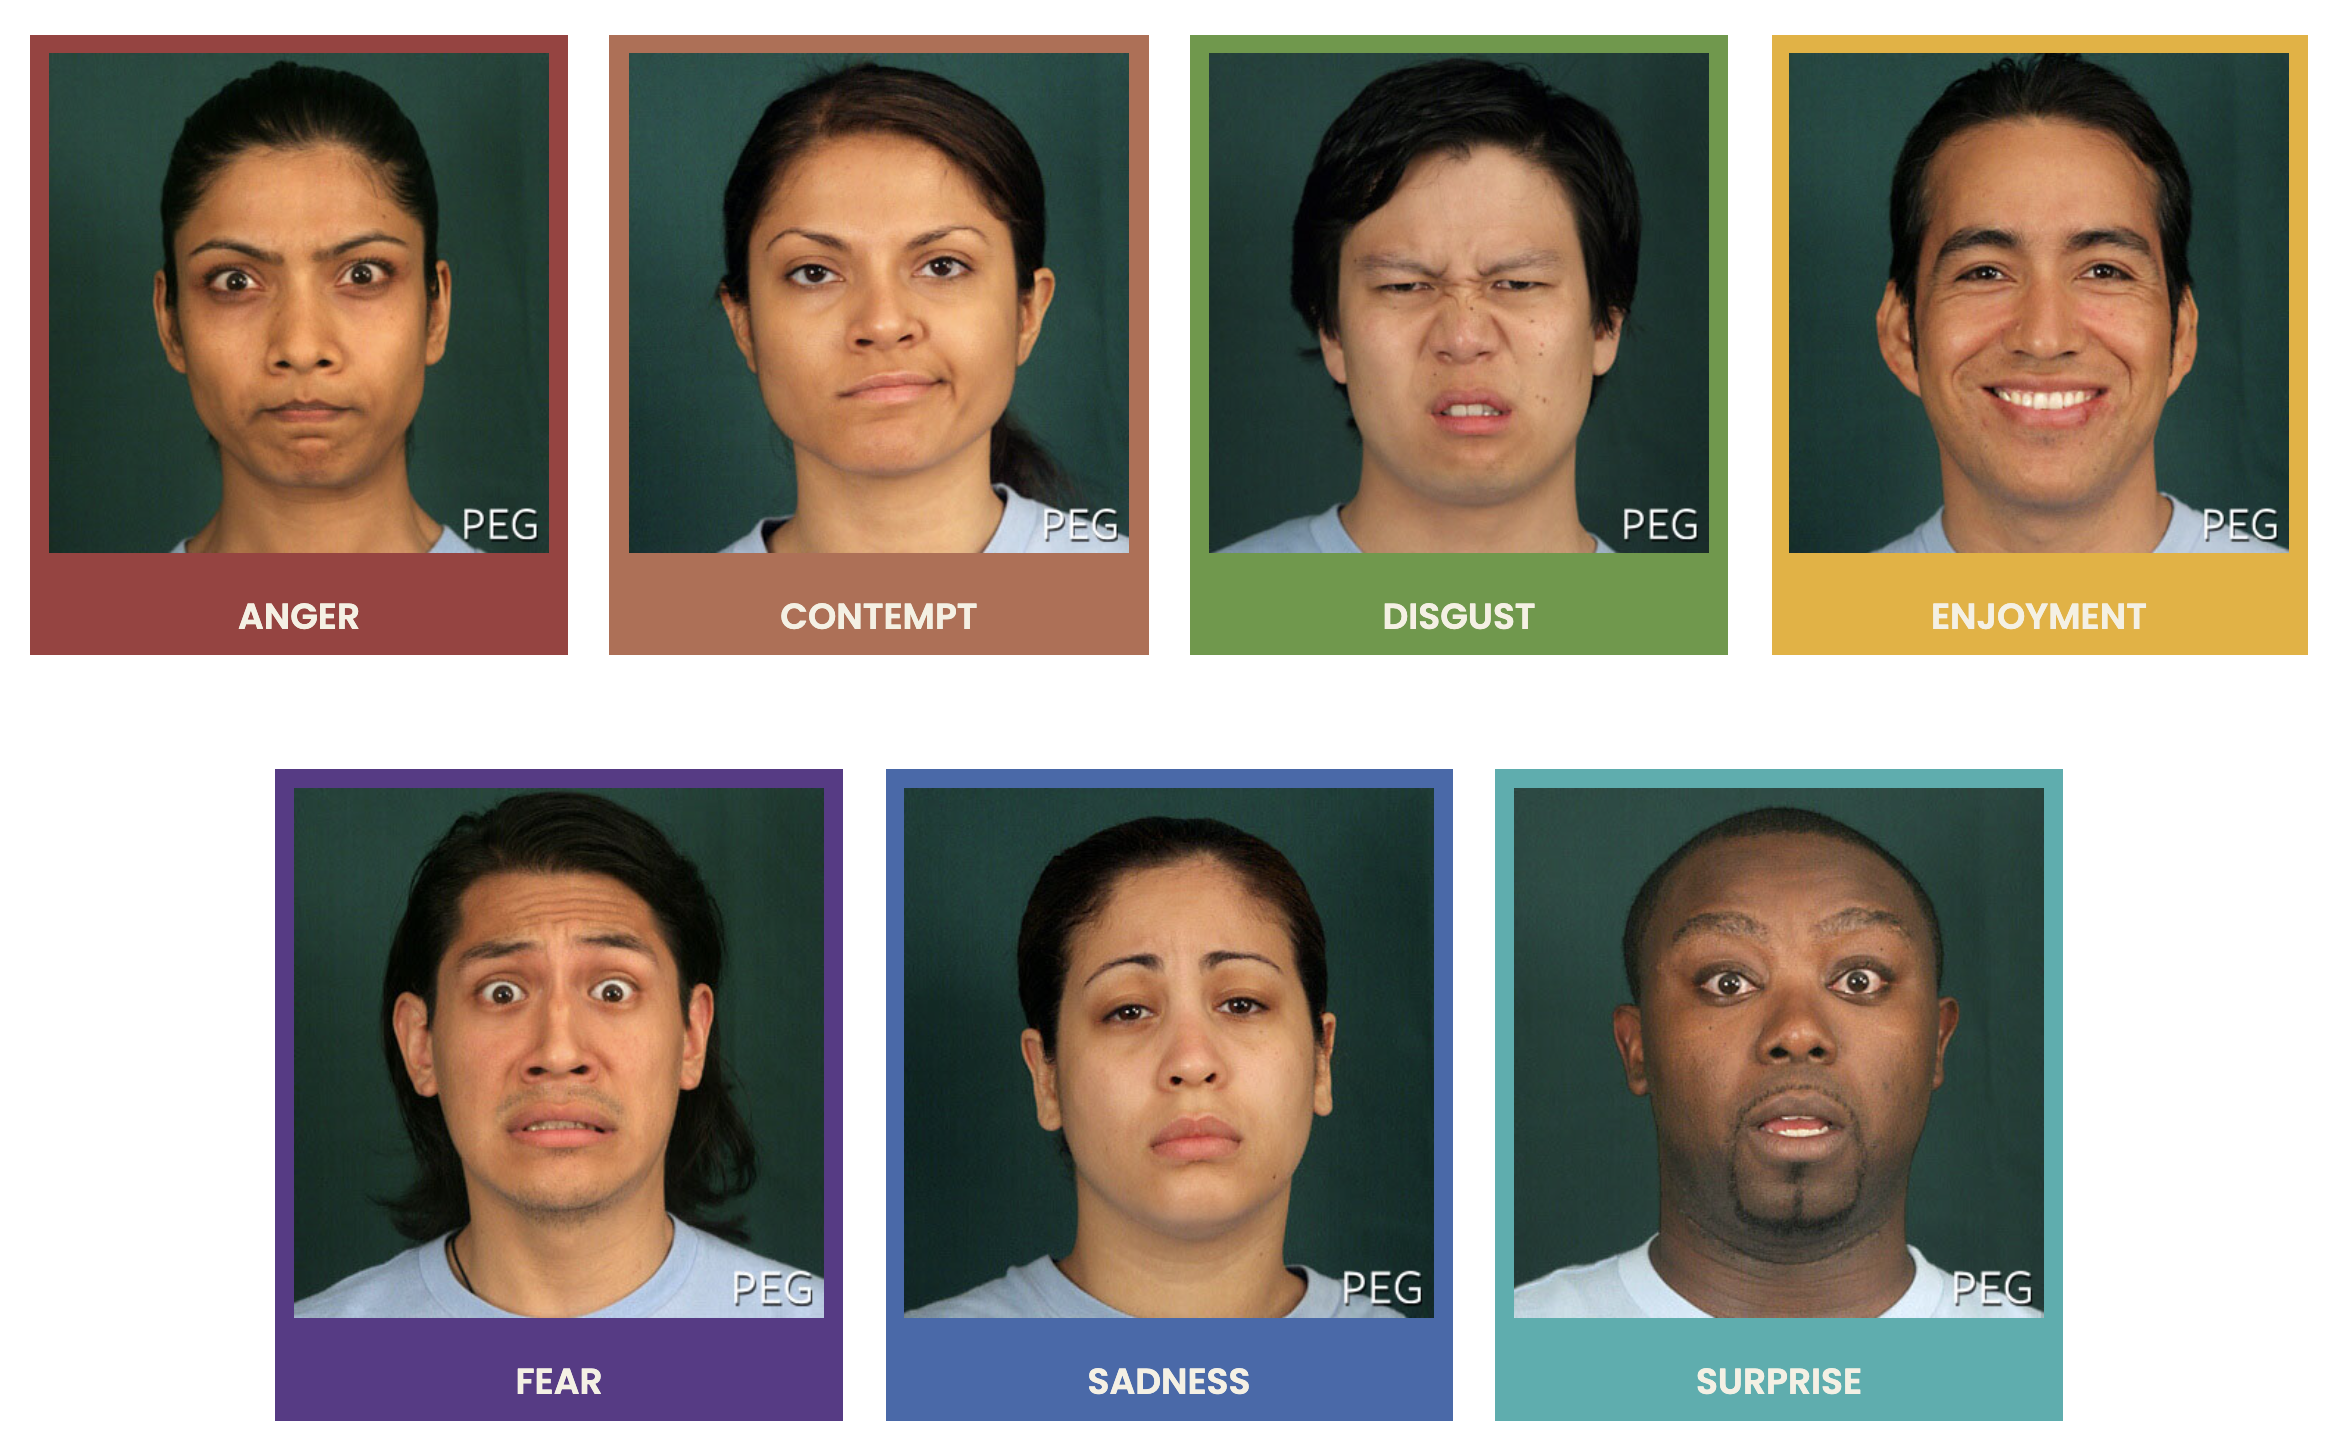
\includegraphics[width=0.5\linewidth]{figures/paul_ekman.png}
    \caption{Paul Ekman's seven basic emotions~\cite{paul_ekman_web}}
    \label{fig:paul_ekman}
\end{figure}

This assumes that emotions are biologically universal and psychologically irreducible. This framework enabled early supervised emotion classification systems by providing a clear labeling scheme and facilitated the construction of benchmark datasets. However, the categorical assumption introduces strong inductive bias; emotions are treated as mutually exclusive and qualitatively distinct.

Subsequent datasets attempted to increase expressive granularity. GoEmotions~\cite{demszky2020goemotionsdatasetfinegrainedemotions}, for example, expanded the label space to 27 emotion categories and allowed multi-label annotation. 

\begin{figure}[H]
    \centering
    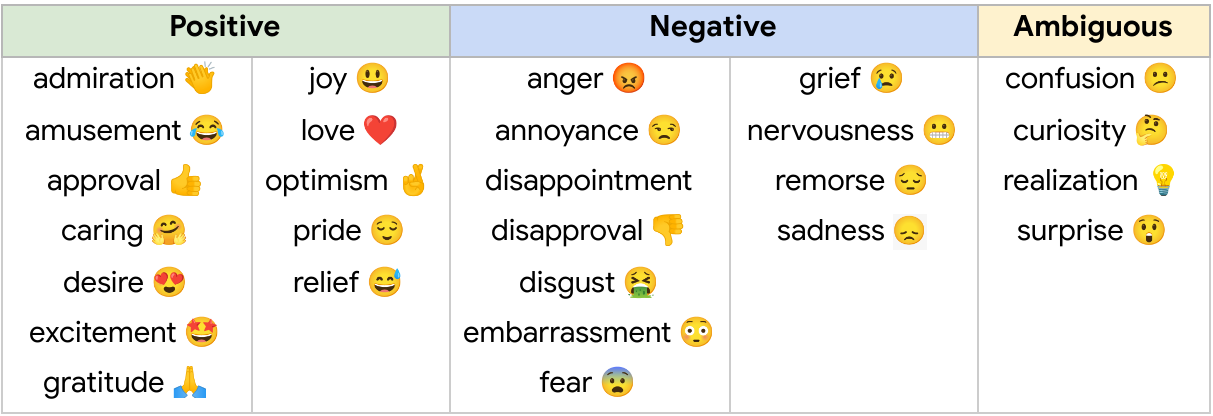
\includegraphics[width=0.8\linewidth]{figures/goemotions.png}
    \caption{GoEmotions taxonomy: 28 emotion categories including ``neutral''.~\cite{goemo}}
    \label{fig:goemotions}
\end{figure}

This enabled us to capture cases where multiple emotions occur in a single utterance. It is reported that emotions cluster by sentiment polarity and intensity, and that many categories exhibit high inter-label correlation. Nevertheless, despite its increased resolution, the dataset still relies on one-hot / sparse multi-hot encodings. Such encodings collapse emotional intensity and compositional structure into discrete indices, preventing the representation of graded transitions. For example, the difference between mild and intense anger cannot be represented, and the blend of emotions, such as bittersweet emotion, is also difficult.

Essentially, discrete labels force the learning problem into a classification regime that cannot capture continuity, geometry, or arithmetic structure. For example, two samples labeled \texttt{joy} may be emotionally distant, while \texttt{joy} and \texttt{contentment} may be emotionally close; yet this structure is invisible to the model itself. These limitations motivate a shift away from purely categorical representations toward continuous emotion spaces.

This problem of the discretised emotion labels is also raised  by Wang and Zong (2021)~\cite{wang-zong-2021-distributed}. They explicitly formalise this by arguing that one-hot emotion labels ignore latent relationships between emotion categories. They observe that emotion calsses are not orthogonal in human perception, but rather exhibit similarity in a gradation manner. More broadly, discrete labeling schemes prioritises  the annotation convenience over the representational adequacy. While it simplify supervision and evaluation, they impose artificial bounadies that obscure the underlying structure of emotions. This mismatch becomes especially problematic when attempting cross-dataset transfer or cross-cultural comparison, where differences in label granularity cannot be reconciled within a purely categorical framework.

These shortcomings have motivated a growing body of work that seeks to represent emotion in continuous spaces, where distance, direction, and magnitude encode affective relationships. By having a representation methods that preserves intensity, similarity and compositionality, we can enable models to capture nuanced emotional variation beyond rigid class boundaries. This transition from discrete labels to continuous emotion spaces is the focus of the next subsection.

\subsection{From Discrete Labels to Continuous Emotion Spaces}

Continuous emotion representations seek to encode emotion as points in a low-dimensional vector space, where distance, direction, and magnitude correspond to psychological relationships. Early psychological models such as the pleasure–arousal–dominance (PAD) framework~\cite{MehrabianRussell1974} formalised emotion along continuous axes, suggesting that emotions differ quantitatively rather than categorically.

\begin{enumerate}
    \item \textbf{Pleasure} represents the hedonic quality of an experience, ranging from unpleasant to pleasant. States such as joy, contentment, and satisfaction occupy the positive end of the pleasure axis, whereas sadness, disgust, and despair lie toward the negative end.
    \item \textbf{Arousal} captures the degree of physiological and cognitive activation associated with an emotional state, ranging from calm or lethargic to excited or agitated. High-arousal states include fear, anger, and excitement, while low-arousal states include relaxation, boredom, or melancholy. 
    \item \textbf{Dominance} reflects the extent to which an individual feels in control of, or overpowered by, a situation. High-dominance states are associated with feelings of agency, confidence, and control (e.g. pride, anger), whereas low-dominance states correspond to submission, helplessness, or vulnerability (e.g. fear, shame). 
\end{enumerate}

Together, these three dimensions define a continuous affective space in which canonical emotion categories correspond to regions rather than points. For example, anger and fear are both negatively valenced and highly aroused, but are separable along the dominance axis; sadness and boredom share low arousal and negative valence, but differ in dominance and intensity. This geometric interpretation naturally accounts for graded emotional intensity, mixed emotions, and smooth transitions between affective states~-- phenomena that are difficult to represent with discrete labels.

\begin{figure}[H]
    \centering
    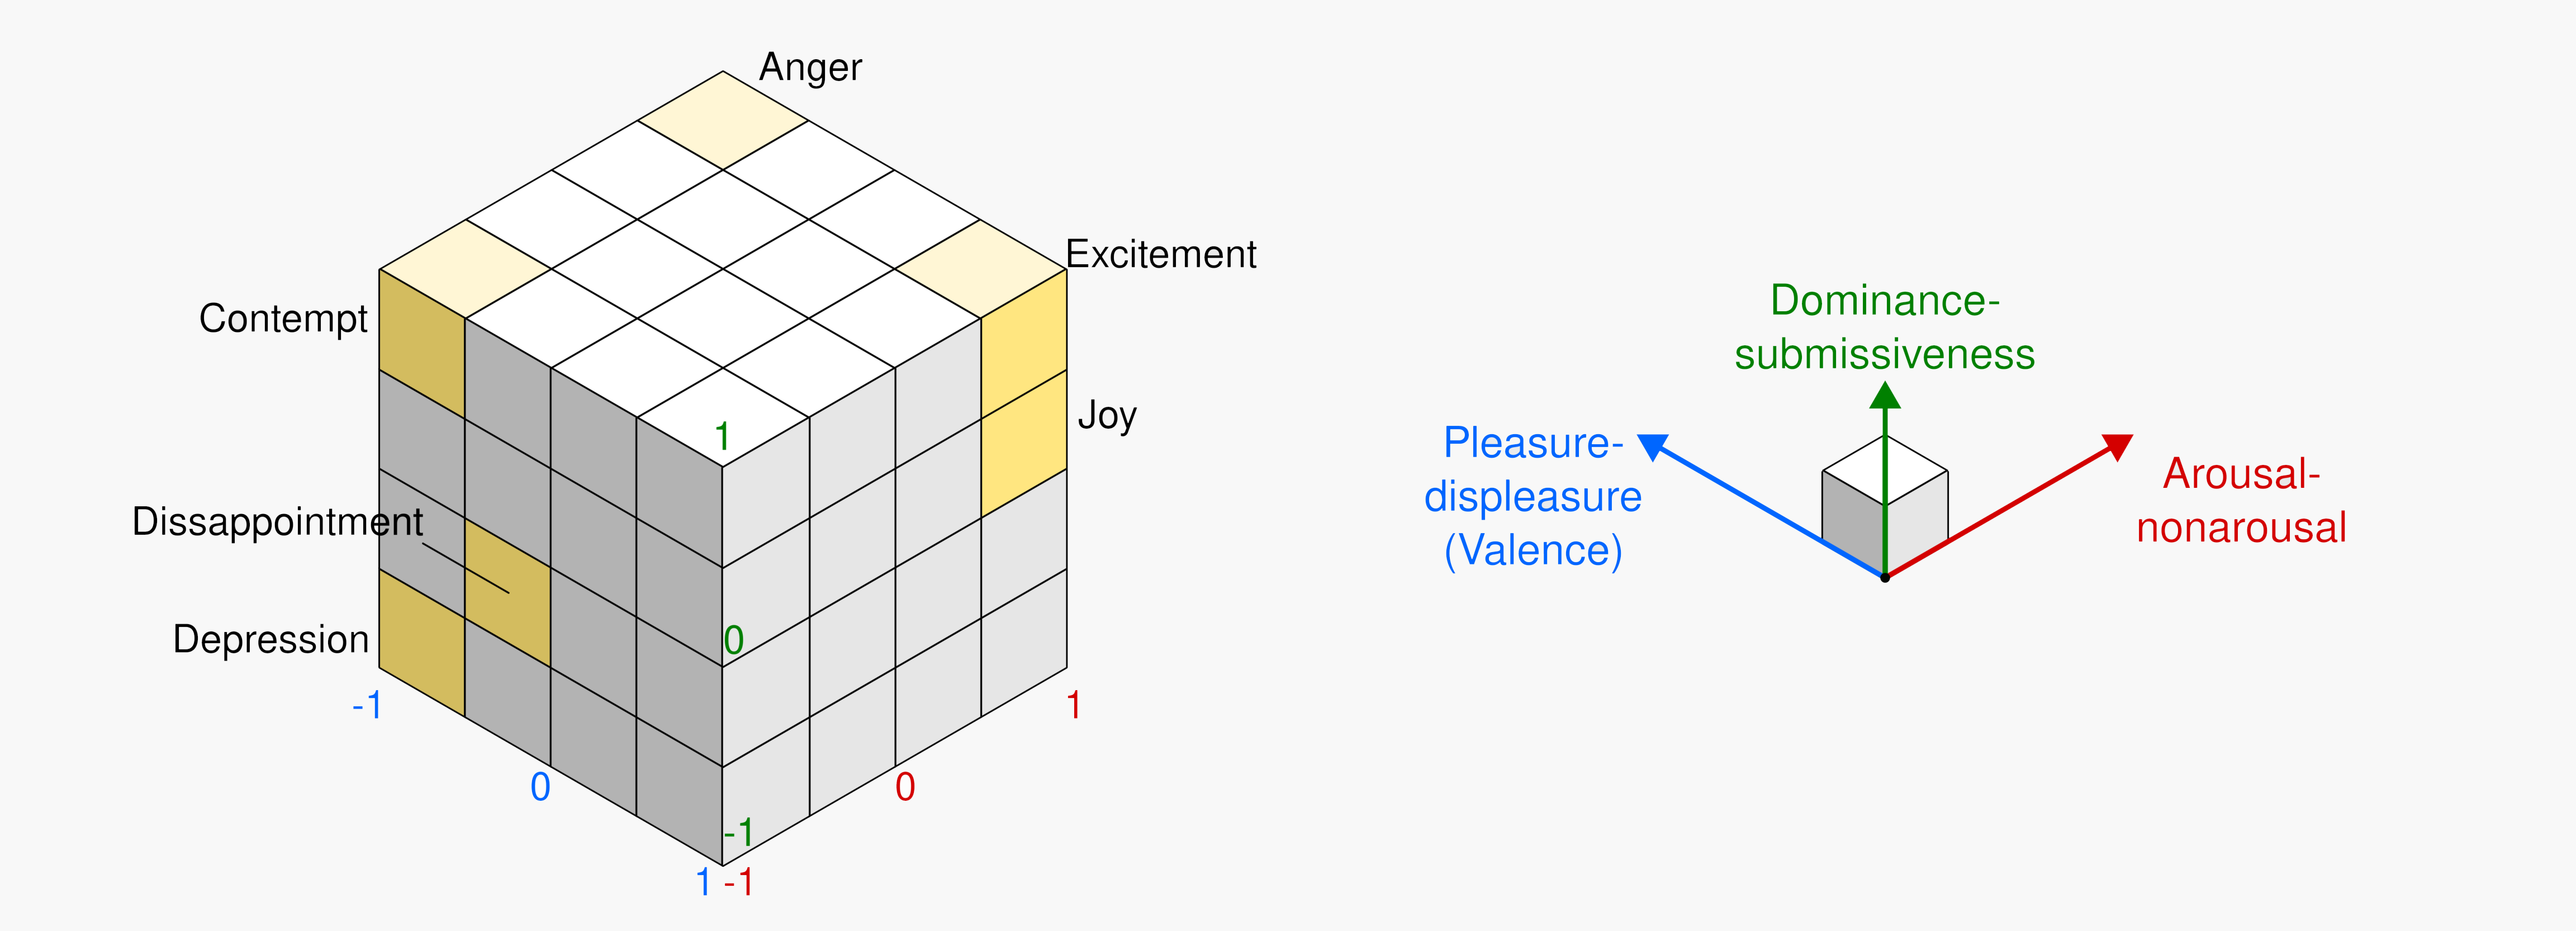
\includegraphics[width=0.8\linewidth]{figures/pad.png}
    \caption{Representation of PAD model done with cubes~\cite{pad}}
    \label{fig:pad}
\end{figure}

Additionally, in the field of affective computing, an explicit attempt to bridge the gap between discrete labels and continuous emotion representations is presented by Buechel et al.~\cite{buechel2021labelagnosticemotionembeddings}. Rather than committing to a single emotion taxonomy, they propose learning \emph{label-agnostic emotion embeddings} that serve as a shared latent representation across heterogeneous annotation schemes, including polarity, basic emotion categories, and affective dimensions such as valence and arousal.

Crucially, emotion labels in this framework are not treated as targets to be predicted directly, but as projections from a common embedding space. Models are trained to map text into this latent affective space, from which multiple label formats can be recovered via lightweight prediction heads. This design enables the learned emotion information to be transferred to another without retraining the full model. Empirically, Buechel et al.\ show that such embeddings preserve prediction quality while supporting cross-dataset generalisation.

Complementary to this, Wang and Zong (2021)~\cite{wang-zong-2021-distributed} focus on learning continuous representations for \emph{emotion categories themselves}. Instead of representing emotion classes as one-hot vectors, they derive distributed emotion embeddings by averaging soft classifier outputs over all instances of a given emotion category. These representations form an emotion space in which distances reflect empirical similarity between emotions as expressed in text. Their results demonstrate that emotion categories cluster by sentiment polarity and intensity, which captures the emotions more faithfully than the conventional semantic word embedding spaces. 

Both of those approaches we looked at enable emotion to be represented as a continuous, low-dimensional structure where each of them corresponds to a region or a direction in a metric space. This perspective aligns closely with psychological theories such as PAD, while remaining grounded in data-driven learning from natural language.

Importantly, representing emotion in continuous spaces shifts the learning problem away from rigid classification toward geometric representation learning. This not only resolves many of the limitations inherent in discrete labels, but also provides a foundation for analysing how emotional information is encoded in vector representations more generally. In particular, it raises the question of whether emotion occupies identifiable subspaces or linear directions within learned embeddings, a topic explored in the following subsection.

\subsection{Linear Structure of Emotion in Word Embedding Spaces} \label{linear_word_embedding}

An important question here is whether the continuous space for emotion is actually reflected in learned language representations. Interestingly, prior to the emergence of LLMs, static word embeddings already exhibited evidence of latent affective organisation, despite being trained without explicit emotional supervision.

Wu and Jiang~\cite{linear_vector_emo} demonstrate that emotional information in word embeddings such as GloVe~\cite{brochier2019global} is not uniformly distributed across dimensions, but instead concentrated along a small number of linear directions. They train a linear autoregressive model to predict continuous emotional valence on annotated narrative data, and show that only a limited subset of embedding dimensions contributes to emotional valence. Interpreting the learned weights reveals that emotional polarity can be captured by a low-dimensional subspace embedded within the full semantic space.

It is also reported that projecting word embeddings into this learned emotion subspace produces a substantially clearer separation between positive and nefative emotion. This indicates that emotion is linearly recoverable even when embeddings are trained without affective objectives. Namely that, emotional meaning is encoded \textbf{geometrically}, rather than a byproduct of lexical associations.

A particularly significant finding is that this projected emotion space preserves \emph{linear compositional structure}. Vector arithmetic over words that contain emotion yields composite affective states, which is also consistent with psychological theories of emotion composition such as Plutchik's wheel of emotions~\cite{plutchik1980emotion}.

\begin{figure}[H]
    \centering
    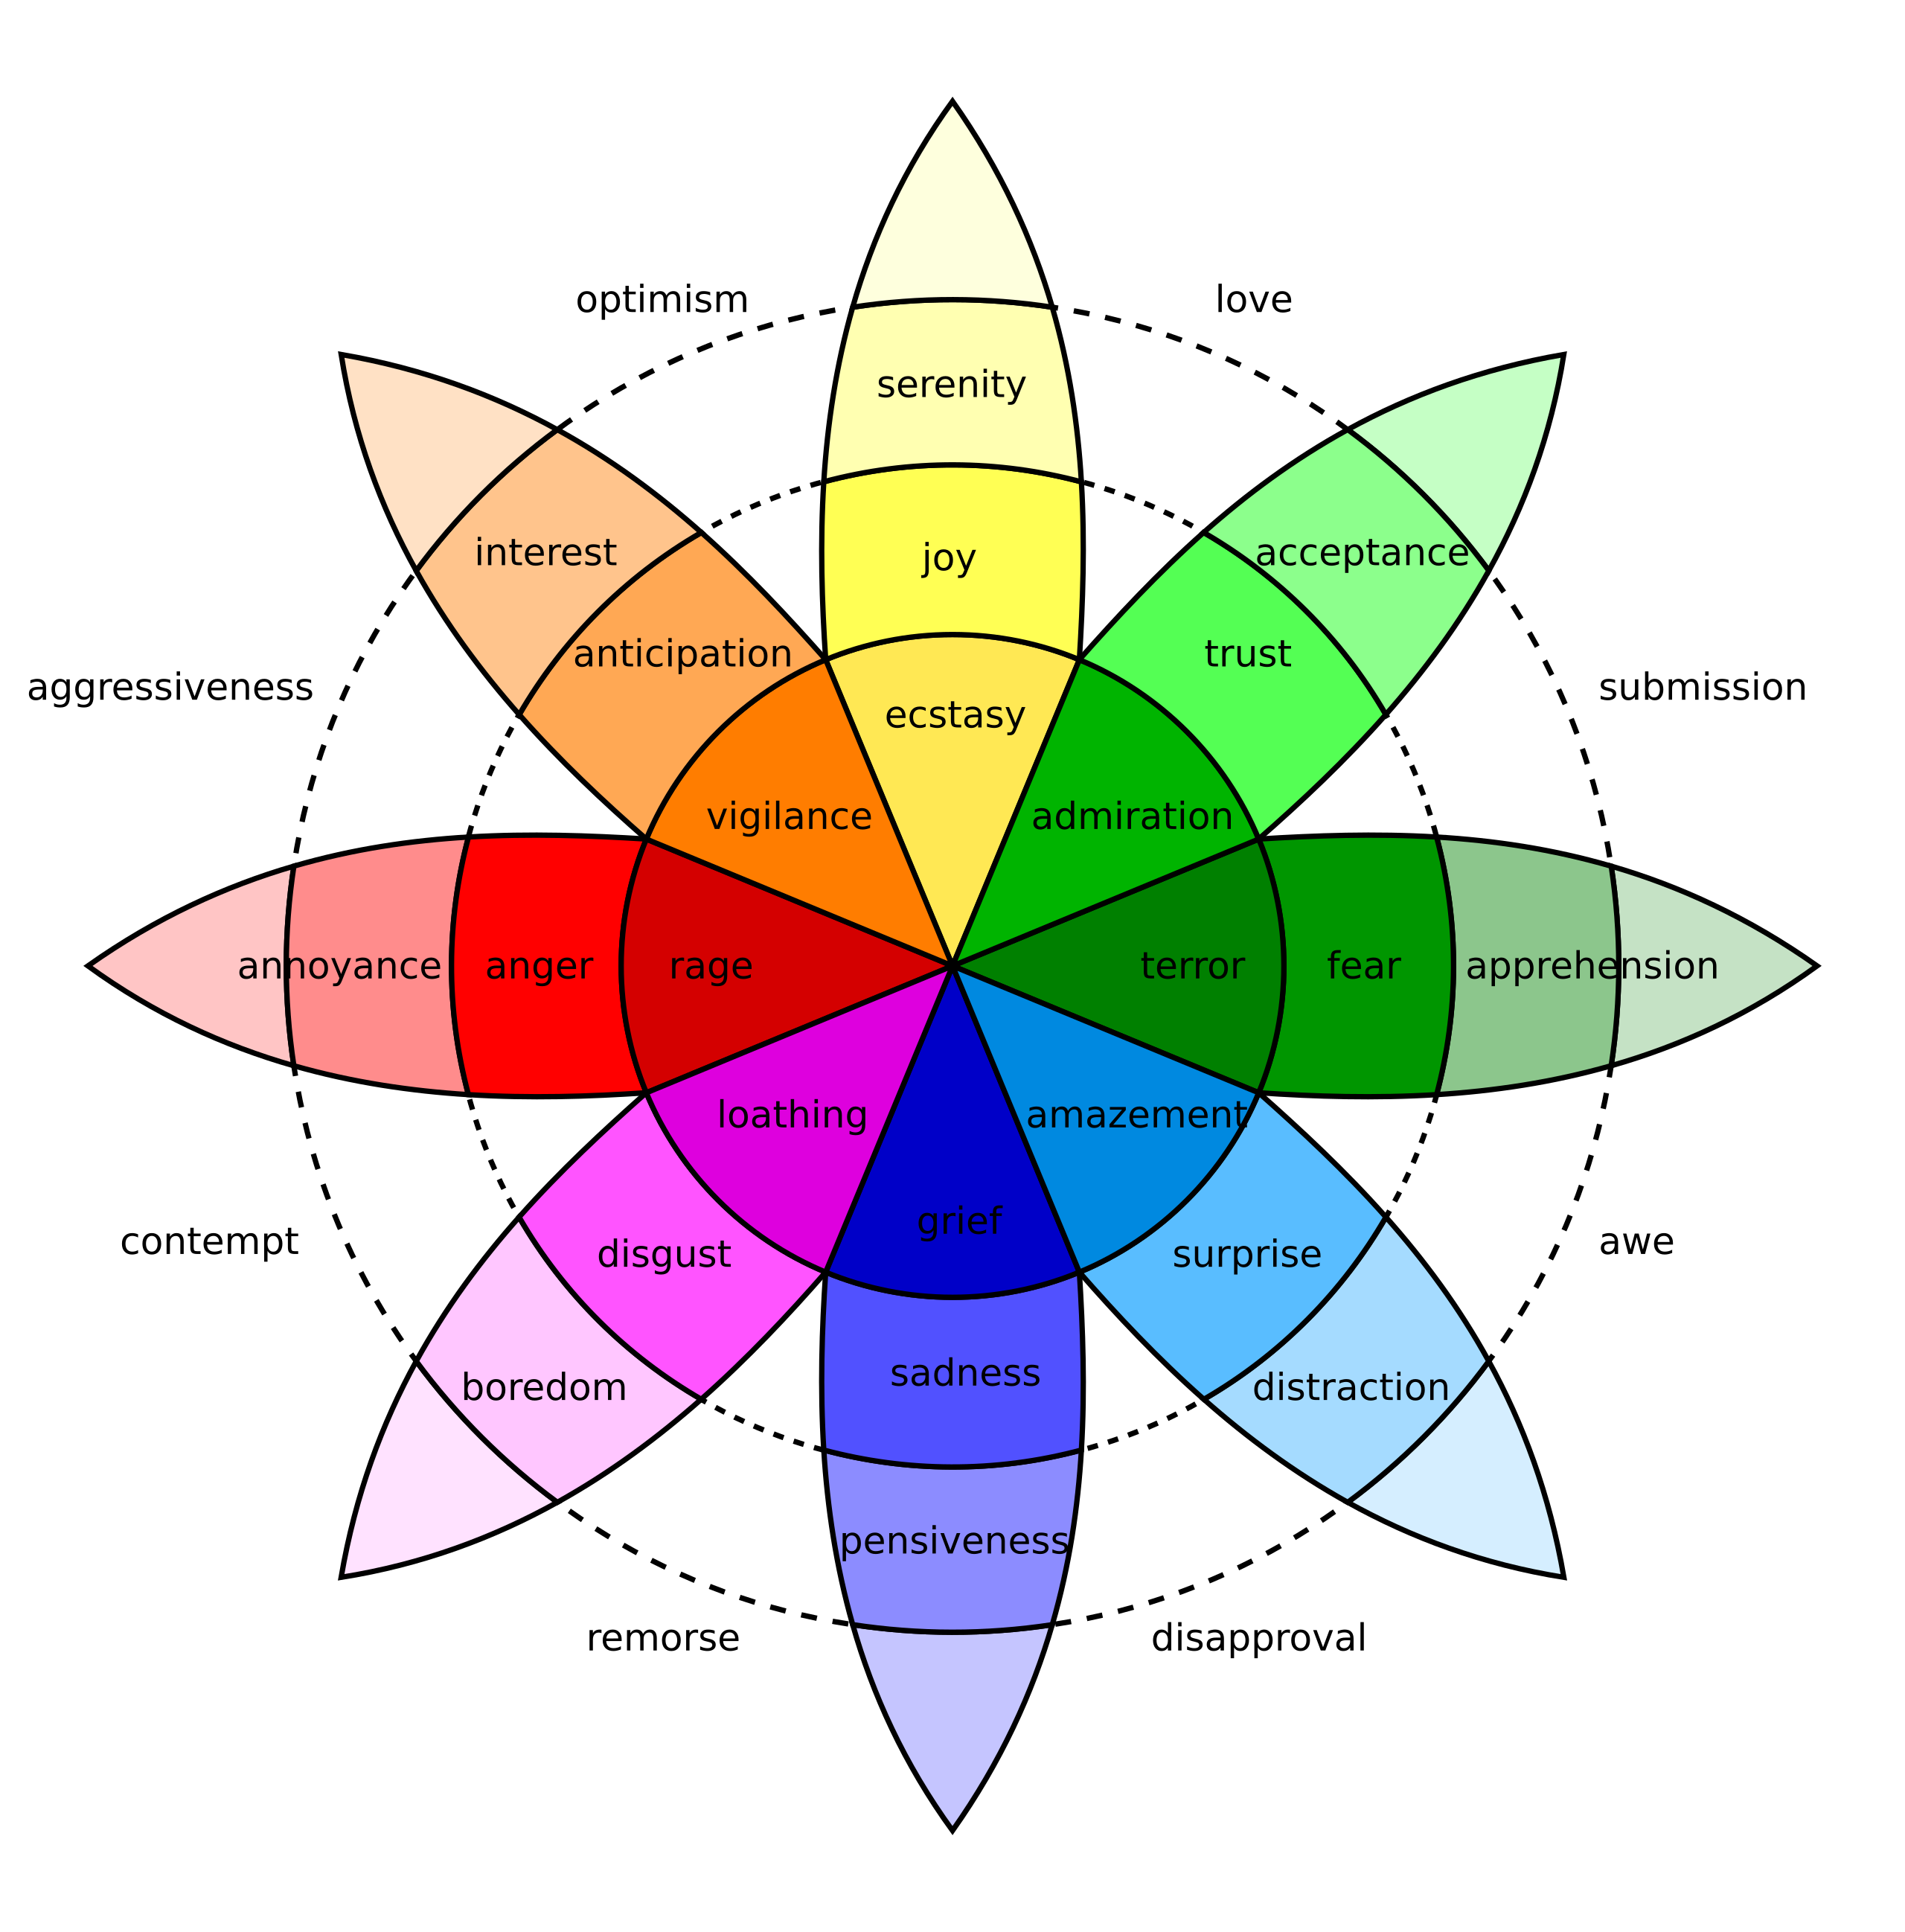
\includegraphics[width=0.5\linewidth]{figures/Plutchik-wheel.png}
    \caption{Plutchik's wheel of emotions: basic emotions are arranged radially, with angular proximity indicating similarity and radial intensity indicating emotional strength.}
    \label{fig:Plutchik}
\end{figure}

For example, the vector sum of \texttt{joy} and \texttt{trust} aligns closely with \texttt{love}, while remaining distant from affectively opposing states such as \texttt{remorse}. This behaviour cannot be captured by categorical representations, but emerges naturally in a continuous, vector-valued framework.

These results indicate that emotion in word embedding spaces is not only continuous but also approximately linear, admitting meaningful projections, directions, and arithmetic operations. As a result, affective similarity, intensity, and composition can be expressed through simple linear operations rather than discrete class boundaries.

Taken together, these findings provide early evidence that emotion is encoded as structured geometry within learned language representations. This establishes a representational bridge between psychological models of emotion and mathematical embedding paradigms. This also motivates further research into how such linear emotional structure scales and evolves in more expressive representation learning systems.

\section{Manipulation of Latent Representations}

To harness these emotion vectors, researchers have explored techniques for directly manipulating internal representations of models.

\subsection{Neuron-Level Emotion Control}

One line of work focuses on exploiting localised affective representations at the neuron level. For instance, Radford et al.\ (2017)~\cite{radford2017learninggeneratereviewsdiscovering} noted a single ``sentiment neuron'' in a byte-level recurrent language model. It has shown that the activation strongly correlates with review polarity and the manipulation of that sentiment neuron directly controls the generated sentiment. Later work shows that modern LLMs contain clusters of neurons selectively responsive to specific emotions. 

Ablation and masking experiments were done by Lee et al.\ (2025)~\cite{lee-etal-2025-large}, and it demonstrates that removing these neurons can selectively impair recognition of particular emotions. This confirms that they play a functional role rather than being incidental correlates. However, there is still a possibility that the model is redundant. For some emotions, performance remains stable after ablation, suggesting overlapping representations and compensatory mechanisms.

Additionally, low-resource fine-tuning methods such as LoRA (Low-Rank Adaptation)~\cite{hu2021loralowrankadaptationlarge} and prefix-tuning operate at a higher level of abstraction but still manipulate latent activations. By injecting small learned vectors into the model we can induce a consistent emotional tone without full retraining. This shows that affective style is encoded in directions that are easy to steer with low-rank updates.

\subsection{Emergent Emotional Subspaces in Large Language Models}

Large language models substantially extend and generalise the affective structure previously observed in static word embeddings (\ref{linear_word_embedding}). Even though models are trained on massive corpora without any emotional information supervision, LLMs acquire rich contextual representations. These models appear to internalise emotion as a continuous and distributed property of their hidden-state geometry.

Recent work provides strong empirical evidence for this claim. Reichman et al.\ (2025)~\cite{reichman2025emotionsartthouunderstanding} show that emotional information in large decoder-only LLMs is organised within a low-dimensional \textbf{emotional manifold} embedded in the activation. 

They analysed hidden states across layers, demonstrated how affective content aligns with a small number of stable latent directions. Importantly, these directions appeared without any explicit emotion supervision, indicating that affective structure is a natural consequence of large-scale language modelling rather than a task-specific artefact. Moreover, the identified emotional subspace is remarkably consistent across domains and languages, suggesting that LLMs internalise a broadly universal affective geometry.

Crucially, this geometry is not merely descriptive. Reichman et al.~\cite{reichman2025emotionsartthouunderstanding} show that small interventions along these latent directions can alter the model's emotional interpretation of an input, while preserving its semantic content. This establishes emotional subspaces as functionally meaningful components of the model's representation space, rather than passive correlates of surface-level sentiment cues. This establishes emotional subspaces to be considered as a functional and meaningful components of the model's representation space.

Complementary evidence comes from neuron-level analyses too. Lee et al.\ (2025)~\cite{lee-etal-2025-large} identify groups of neurons whose activations selectively track specific basic emotions in large instruction-tuned models. Emotional information is broadly distributed, but certain neurons constantly exhibit disproportionately strong responses to particular affective states. Further ablation experiments revealed that suppressing these neurons can significantly degrade emotion recognition performance for some emotions. This provides a causal evidence that emotional information is actively processed rather than epiphenomenal.

Taken together, these findings suggest that emotion in LLMs is best characterised as an emergent, low-dimensional subspace embedded within high-dimensional contextual representations. Emotional meaning is not localised to single units, nor reducible to discrete labels; instead, it occupies a structured region of stable latent space. This emergent affective geometry provides the representational foundation that enables direct control of emotional behaviour through linear interventions, which we discuss next.

\subsection{Steering Latent States with Linear and Continuous Control Vectors}

If emotional meaning in LLMs is encoded as directions or subspaces within latent representations, a natural consequence is that affective behaviour should be directly controllable by intervening along those directions. This observation has motivated a line of work on \textbf{latent steering}, in which linear and continuous control vectors are applied directly to internal activations during inference.

An early and influential approach is Plug-and-Play Language Models (PPLM)~\cite{dathathri2020plugplaylanguagemodels}, combines a frozen language model with an external attribute model (e.g.\ a sentiment classifier) and performs gradient ascent on the hidden states to increase the likelihood of a desired attribute. Effectively, this method introduces a small \textbf{sentiment vector} into the latent representation, biasing generation toward positive or negative emotion without modifying the model's weights. Although originally framed as a controllable generation technique, PPLM implicitly relies on the assumption that affective attributes correspond to approximately linear directions in latent space.

More recent work makes this assumption explicit and removes the need for iterative optimisation. Anthropic's \textbf{Contrastive Activation Addition} (CAA)~\cite{caa} directly intervenes in a model's internal activations using precomputed \textbf{steering vectors}. These vectors are obtained by collecting large sets of positive and negative examples of a target behaviour or attribute and averaging the differences in their intermediate representations. The resulting vector captures a direction in latent space that causally corresponds to the desired attribute. During inference, adding this vector to the residual stream steers model behaviour in a predictable manner, while leaving the model parameters unchanged.

A key advantage of CAA is its simplicity and interpretability. The intervention is linear, and the strength of the effect can be modulated continuously by scaling the steering vector with a scalar coefficient. Moreover, multiple steering vectors can be combined additively, enabling compositional control over several attributes simultaneously. In contrast to prompt engineering or fine-tuning, such interventions operate directly on the model's internal state and often yield more precise and robust control, particularly for abstract properties such as sentiment or emotional tone. 

Crucially, steering latent states does not only affect surface-level lexical choices. Injecting affective control vectors at intermediate layers can alter the model's internal interpretation of emotional context, changing how emotional cues are integrated and propagated through the network. This supports the view that emotion in LLMs functions as a global latent variable, rather than as a property tied to individual tokens or outputs.

As conclusion, latent steering methods such as PPLM and CAA provide strong evidence that emotional subspaces in LLMs are not only emergent and structured, but also causally actionable. Manipulating affective behaviour through simple linear interventions reinforces the interpretation of emotion as a continuous geometric representation space. It further bridges descriptive analyses of emotional geometry with concrete mechanisms for controlling model behaviour.

\subsection{Causal Evidence for Linear Sentiment and Emotion Directions}

The existence of affective directions in representation space can be shown by linear probes or dimension reduction, however, it is still doubtful if they actually play a causal role in model behaviour. Recent work provides strong evidence that emotion directions in LLMs are not only linearly recoverable, but also functionally necessary and sufficient for affective reasoning.

Hollinsworth et al.\ (2024)~\cite{hollinsworth-etal-2024-language} show that sentiment in LLMs is encoded along a single dominant linear direction in contextual embeddings. They perform directional ablations and interventions, demonstrating that removing / suppressing this sentiment direction causes systematic degradation in downstream emotion-sensitive tasks such as emotion classification. Conversely, injecting the same direction into neutral contexts induces predictable shifts in model outputs. This bidirectional manipulation provides an evidence that the emotion direction is actively used by the model rather than being a passive correlate.

Importantly, affective competence in LLMs does not depend on explicit fine-tuning for emotion-related tasks. Broekens et al.\ (2023)~\cite{broekens2023finegrainedaffectiveprocessingcapabilities} demonstrate that off-the-shelf LLMs such as ChatGPT can map text to precise valence–arousal–dominance (VAD) values and detect fine-grained emotional cues using prompting alone. This sugegsts that continuous affective representations are already embedded in the latent space as part of general language understanding. This is a strong evidence that interpretes emotion as a pre-verbal latent variable, rather than a task-specific output format.

At larger scales, evidence further indicates that emotional representations are not flat but hierarchically structured. Zhao et al.\ (2024)~\cite{zhao2025emergencehierarchicalemotionorganization} observe that very large models (more than 405 billion parameters) develop tree-like emotion representations, where basic affective states branch into more specific emotions. Models featuring a more consistent hierarchical affective geometry demonstrate enhanced emotion recognition capabilities and increased persuasive effectiveness in negotiation scenarios. This directly links the internal structure of emotional expression to functional behaviour.

These findings converge on a causal interpretation of affective geometry in LLMs. Removing emotion directions impairs affective reasoning, while injecting them predictably alters behaviour. Moreover, emotional information is not confined to isolated tokens or neurons, but is accumulated and summarised across layers into global latent variables that shape general affective capabilities of models.

In conclusion, there is a principled foundation for vector-based manipulation of emotion, which enables us to express emotional nuance through numeric operations on embeddings rather than token-level substitutions. This causal grounding is essential for our project that seeks to control and align emotional behaviour in large language models.

\section{Reasoning Beyond Token Space}

\subsection{Limitations of Token-Based Reasoning}

Conventional LLMs reason in token space. Because inputs are projected onto the discrete boundaries humanity drew as ``vocabulary,'' fine affective nuance and embodied subtleties are irretrievably lost during that projection, and what remains in one output language may differ from what remains in another. To adjust tone, one often uses prompt engineering or instruction tuning (``Please answer politely,'' etc.), but adherence is uncertain and fine-grained control is difficult. Other countermeasures include supervised fine-tuning to internalise a style, or label-conditioned generation (e.g.\, adding \texttt{<joy>} \texttt{<sad>}), but fine-tuning is costly and switching between styles is inflexible; label conditioning also cannot capture complex blends of nuance.

Beyond affective control, the same limitation applies to reasoning itself. Autoregressive language models do not take token functionality into account in its generation process. Even if the token carries significant reasoning content, it will be allocated approximately same computational budget as grammartical tokens like \texttt{a} or \texttt{is}. As a result, only a small subset of internal states carries the actual inferential work, and most of the tokens in explicit reasoning traces do not contribute to the underlying computation.

Recent works show this disconnectivity between the surface output tokens and internal reasoning process. Pfau et al.\ (2024)~\cite{pfau2024lets} demonstrate that transformers can perform non-trivial hidden computation even when output tokens are semantically uninformative. For example, inserting filler or pause tokens (carry no explicit meaning) somehow measurably improve performance on reasoning tasks. This suggests that the essential computation is carried by latent activations rather than by the emitted tokens themselves. Token generation only a communicative language constraint around an internal process.

The inefficiency of token-based reasoning becomes more apparent when reasoning is explicitly verbalised. Chain-of-thought prompting improves performance in many tasks, however \textbf{it requires the model to externalise intermediate states into natural language, even when those states are not naturally linguistic}. As argued by Hao et al.\ (2025)~\cite{hao2025traininglargelanguagemodels}, language is optimised for communication rather than for computation. Forcing reasoning to unfold within the constraints of a discrete vocabulary introduces unnecessary overhead and distortion. Many reasoning tokens exist not because they are required for inference, but because they are required for human readability.

From this perspective, explicit verbalisation constitutes a form of lossy compression for an affective reasoning as discussed in the previous section. The continuous and high-dimensional internal states during inference must be projected onto a discrete and culturally contingent token space, which flattens distinctions that are visible for computation but words-level invisible. This compression is problematic for affective computing, because emotion structure is inherently graded, which is resistant to precise lexicalisation.

Taken together, these observations suggest that token space not a substrate of reasoning, but rather an interface. While it provides a convenient medium for communication and supervision, it is suboptimal for internal computation. This motivates a growing line of work that seeks to decouple reasoning from explicit token generation. Computation can proceed without the constraints imposed by language.

\subsection{Reasoning in Continuous Latent Space}

Motivated by the observation that reasoning is primarily carried by latent activations rather than surface tokens, a growing body of work has explored \textbf{implicit} forms of chain-of-thought. The central idea is to retain the intermediate reasoning within the model's hidden state, so that we can benefit from the multi-step reasoning while avoiding the distortions introduced by forcing intermediate states into natural language.

Early implicit chain-of-thought approaches aim to internalise reasoning traces by gradually removing explicit reasoning tokens during training, encouraging the model to perform the same computation silently in its latent space. More recent methods go further by explicitly allocating computation to continuous latent representations that replace textual reasoning steps altogether. In these models, reasoning unfolds as a sequence of hidden-state transitions, while the output layer is used only to produce the final answer.

A representative work is \textbf{CODI} (Compressing Chain-of-Thought into Continuous Space via Self-Distillation)~\cite{shen2025codicompressingchainofthoughtcontinuous}. This approach compresses explicit chain-of-thought trajectories into a compact sequence of continuous latent states, and by distilling a teacher model that produces explicit reasoning traces, CODI trains a student model to reproduce the same reasoning outcome using a shorter sequence of latent vectors. This demonstrates that the information carried by textual reasoning can be encoded more efficiently in continuous space, without requiring token-level supervision at inference time.

A more radical approach is proposed by \textbf{Coconut} (Chain of Continuous Thought)~\cite{hao2025traininglargelanguagemodels}. Rather than compressing explicit reasoning traces, Coconut modifies the inference procedure itself by feeding the model's last hidden state back as the next input embedding. In this way, reasoning unfolds entirely within continuous latent space and there is no need of intermediate textual tokens at all. However, because Coconut relies primarily on answer-level supervision, the resulting latent trajectories can be unstable when extended to deeper reasoning chains, which we discuss in the next subsection.

\subsection{Implicit and Continuous Chain-of-Thought}

However, there is one challenge that purely implicit reasoning introduces. When multiple latent reasoning steps are chained together without sufficient structural constraints, the latent representations can collapse into homogeneous states. This phenomenon is often referred to as \textbf{latent collapse}, which undermines the model's ability to maintain distinct intermediate representations.

\textbf{SIM-CoT} (Supervised Implicit Chain-of-Thought)~\cite{wei2025simcot} addresses this limitation by introducing step-level supervision during training. Instead of supervising only the final answer or the overall reasoning trajectory, SIM-CoT attaches an auxiliary decoder that forces each latent reasoning step to predict a corresponding explicit reasoning phrase. This alignment ensures that each latent vector encodes distinct, semantically meaningful content, preventing homogenisation and improving stability. Crucially, the auxiliary decoder is used only during training and is removed at inference, allowing the model to retain the efficiency of silent latent reasoning while benefiting from structured supervision. Empirically, SIM-CoT substantially improves both performance and robustness over earlier latent reasoning models, including Coconut-style architectures.

It attaches an auxiliary decoder that forces each latent reasoning step to predict a corresponding explicit reasoning phrase, which ensures that each latent vector to encoded semantically meaningful content. This substantially improves both performance and robustness over earlier latent reasoning models, including Coconut-style architectures. Importantly, the auxiliary decoder is used only during training and is removed at inference, allowing the model to retain the efficiency of silent latent reasoning while benefiting from structured supervision.

These approaches demonstrate that chain-of-thought need not be realised as a sequence of discrete tokens. Reasoning can be instead implemented as a controlled trajectory through continuous latent space, with explicit language serving primarily as a training scaffold or interpretability aid.  Implicit and continuous chain-of-thought models provide a natural foundation for studying how emotions may be represented and manipulated within latent reasoning processes.

\subsection{Implications for Affective Representation}

The developments reviewed above suggest a converging picture of representation and computation in LLMs. As discussed in earlier sections, emotions are not confined to discrete labels or lexical choices but it rather emerges as a continuous structure within latent space. At the same time, recent advances in implicit chain-of-thought demonstrate that reasoning itself can be implemented as a trajectory through that same latent space, without requiring intermediate symbolic tokens.

These findings summarises to the fact that emotion need not be treated as separate components at the level of surface language. Instead, it appears to be grounded in shared latent representations that evolve over the course of inference. From this perspective, emotional information may constitute an integral part of the internal reasoning state itself, shaping how intermediate representations are formed and propagated.

Importantly, this possibility remains largely unexplored. Although latent reasoning frameworks have demonstrated improved eff expressivity for logical and mathematical tasks, their implications for affective representation have not been systematically examined. Whether emotional dimensions align or interact with latent reasoning trajectories is an open question. Addressing this gap requires moving beyond token-level analysis and considering emotion as a first-class component of latent computation rather than as a stylistic attribute.

These considerations motivate the investigation in the following chapters. Rather than treating emotion as an external label or an output constraint, we explore the hypothesis that affective states can be represented within continuous latent spaces that underlie reasoning itself. By doing so, we aim to better understand how emotional meaning may be re-expressed when language is no longer the primary medium of inference.

%%%%%%%%%%%%%%%%%%%%%%%%%%%%%%%%%%%%